\documentclass[10pt]{beamer}

% used Commands for installing everything needed + VSCode Packages

% sudo apt install texlive-latex-extra
% sudo apt -y install texlive-lang-german
% sudo apt install chktex
% sudo apt install latexmk

% https://hartwork.org/beamer-theme-matrix/

%Style
\mode<presentation>{
    %Theme
    %\usetheme{default}
    %\usetheme{AnnArbor}
    %\usetheme{Antibes}
    %\usetheme{Bergen}
    %\usetheme{Berkeley}
    %\usetheme{Berlin}
    %\usetheme{Boadilla}
    %\usetheme{CambridgeUS}
    %\usetheme{Copenhagen}      ||||||
    %\usetheme{Darmstadt}
    %\usetheme{Dresden}
    %\usetheme{Frankfurt}
    %\usetheme{Goettingen}
    %\usetheme{Hannover}
    %\usetheme{Ilmenau}
    %\usetheme{JuanLesPins}
    %\usetheme{Luebeck}
    %\usetheme{Madrid}
    %\usetheme{Malmoe}           ||||||||||||||
    %\usetheme{Marburg}
    %\usetheme{Montpellier}
    %\usetheme{PaloAlto}
    %\usetheme{Pittsburgh}
    %\usetheme{Rochester}
    %\usetheme{Singapore}
    %\usetheme{Szeged}
    %\usetheme{Warsaw}
    \usetheme{metropolis}                          %||||||||||||||||||||||||||||||||
    
    %Farb-Theme
    %\usecolortheme{albatross}
    %\usecolortheme{beaver}             ||||||||||||||||||||||||||||
    %\usecolortheme{beetle}
    %\usecolortheme{crane}
    %\usecolortheme{dolphin}      |||||||
    %\usecolortheme{dove}
    %\usecolortheme{fly}
    %\usecolortheme{lily}
    %\usecolortheme{orchid}
    %\usecolortheme{rose}
    %\usecolortheme{seagull}
    %\usecolortheme{seahorse}
    %\usecolortheme{whale}
    %\usecolortheme{wolverine}

    %\setbeamertemplate{footline} % Fußzeile entfernen
    %\setbeamertemplate{footline}[page number] % Fußzeile entfernen und durch Folien-Zahl ersetzen

    %\setbeamertemplate{navigation symbols}{} % Navigations-Symbole entfernen
}

%Packages
\usepackage[utf8]{inputenc} %Deutsche Umlaute
\usepackage[ngerman]{babel} %Deutsche Sprache
\usepackage{graphicx}       %für Bilder
\usepackage{booktabs}       %für \toprule \midrule \bottomrule in Tabellen

\renewcommand{\baselinestretch}{1} 
%\geometry{top=100mm}
%\addtolength{\topmargin}{10pt}
%Einstellungen der Präsi
\title{Speedcubing}
\author{Kimi Löffel}
\institute[Bbc]{ICT Berufsbildungscenter}
\date{\today}



\begin{document}

    %Titelseite
    \begin{frame}
        \titlepage{}
    \end{frame}



    %Inhaltsverzeichnis
    \begin{frame}{Inhalt}
        \vspace{20pt}
        \tableofcontents
    \end{frame}



    \section{What is it?}

        %What is Speedcubing
        \begin{frame}{What is it?}
            \begin{itemize}
                \pause{}
                \item Speedsolving a puzzle \pause{}
                \item Collecting Puzzles \pause{}
                \item Modders
            \end{itemize}
        \end{frame}
    


    \section{Puzzles}
        \subsection{WCA}
        
            \subsubsection{What is the WCA?}

                %What is the WCA
                \begin{frame}{What is the WCA}
                    \begin{itemize}
                        \pause{}
                        \item World Cube Association \pause{}
                        \item Organizes Competitions \pause{}
                        \item Award official records
                    \end{itemize}
                \end{frame}

            \subsubsection{WCA puzzles/events}

                %All WCA puzzles and events
                \begin{frame}{WCA puzzles and events}
                    \begin{columns}[c] 
                        \column{.27\textwidth} %linke spalte
                            \begin{itemize}
                                \item<1-> 2$\times$2$\times$2 
                                \item<2-> 4$\times$4$\times$4 
                                \item<3-> 5$\times$5$\times$5 
                                \item<4-> 6$\times$6$\times$6 
                                \item<5-> 7$\times$7$\times$7 
                                \item<6-> 3$\times$3$\times$3 
                                \item<7-> 3$\times$3$\times$3 BLD 
                                \item<8-> 3$\times$3$\times$3 FMC 
                                \item<9-> 3$\times$3$\times$3 OH 
                            \end{itemize}
                        \column{.3\textwidth} % mittlere Spalte
                            \begin{itemize}
                                \item<10-> Clock 
                                \item<11-> Megaminx 
                                \item<12-> Pyraminx 
                                \item<13-> Skewb 
                                \item<14-> Square-1 
                                \item<15-> 4$\times$4$\times$4 BLD 
                                \item<16-> 5$\times$5$\times$5 BLD 
                                \item<17-> 3$\times$3$\times$3 Multi-BLD
                            \end{itemize}
                        \column{.25\textwidth} %rechte spalte 1

                            \begin{figure}
                                \visible<10->{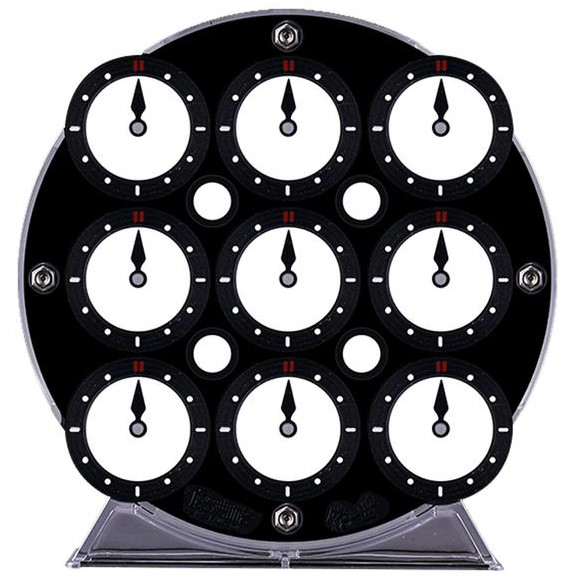
\includegraphics[width=0.6\textwidth]{assets/clock.jpg}}
                                \visible<11->{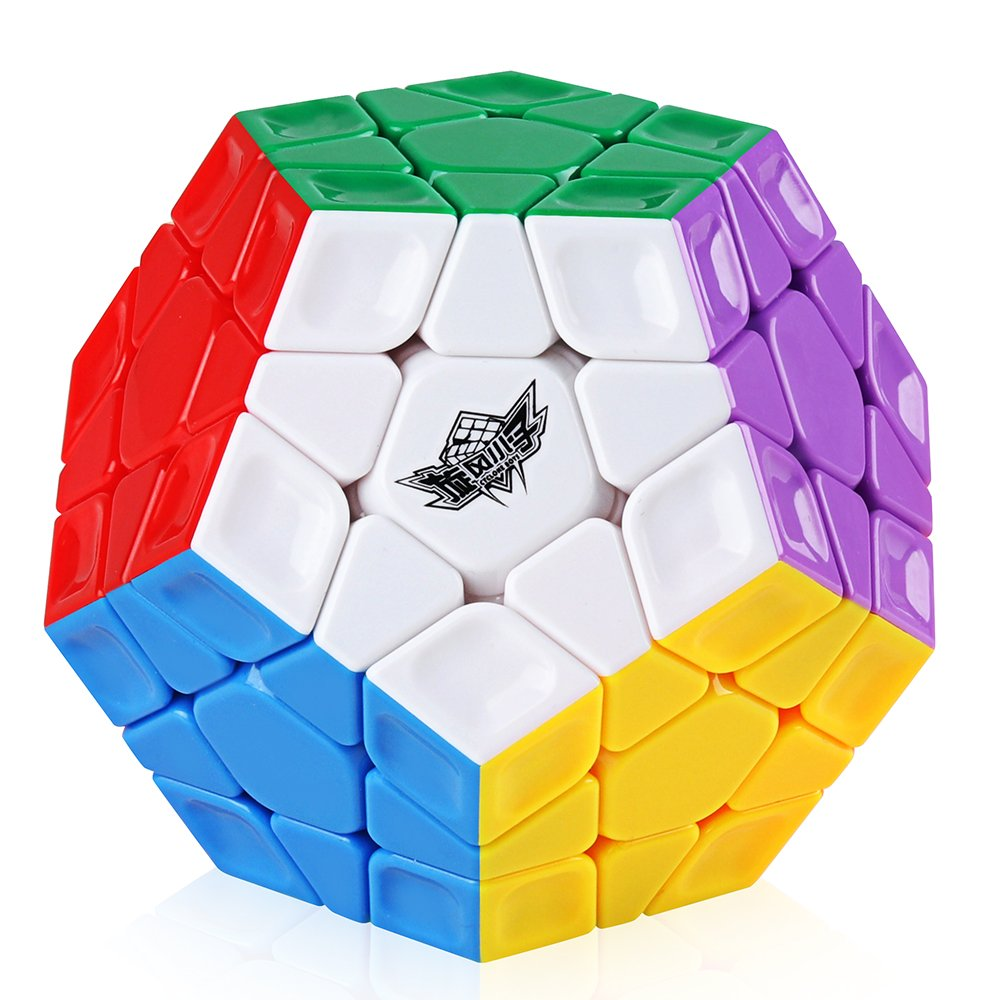
\includegraphics[width=0.6\textwidth]{assets/mega.jpg}}
                                \visible<12->{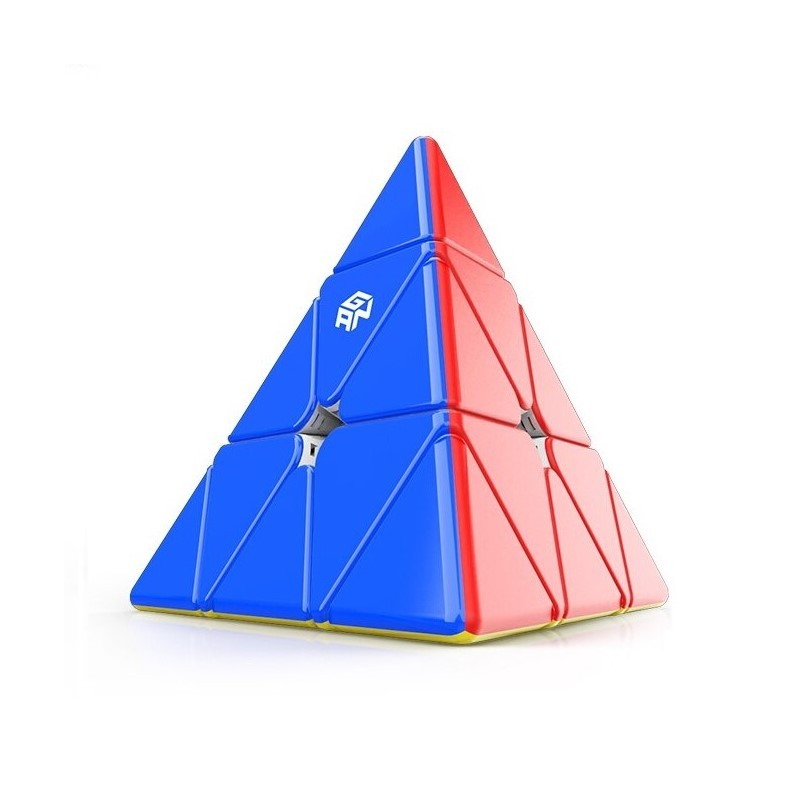
\includegraphics[width=0.7\textwidth]{assets/pyra.jpg}}
                            \end{figure}
                        \column{.25\textwidth} %rechte spalte 2
                            \begin{figure}
                                \visible<13->{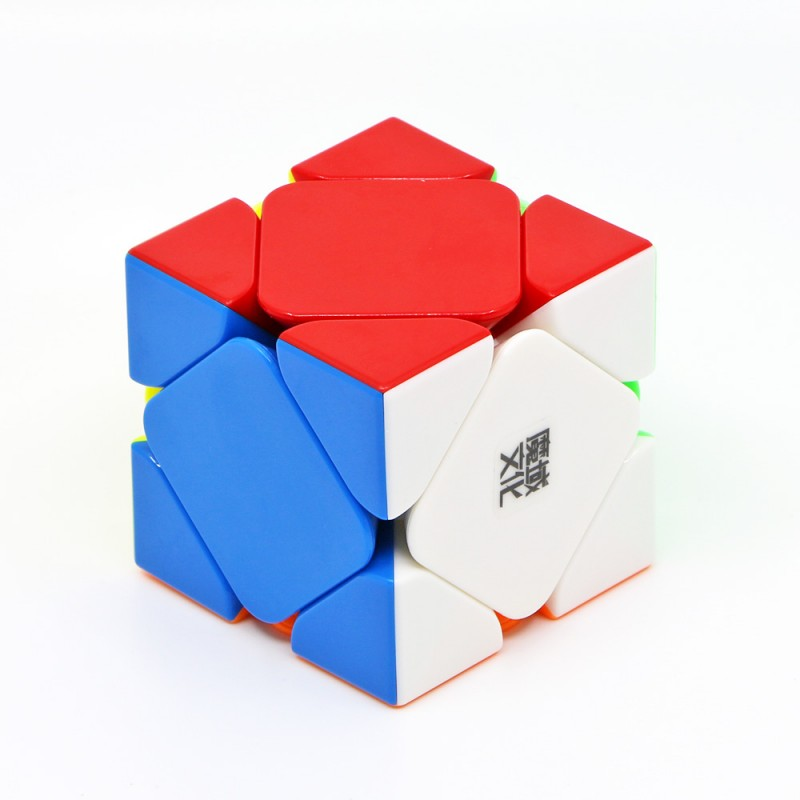
\includegraphics[width=0.9\textwidth]{assets/skewb.jpg}} 
                                \visible<14->{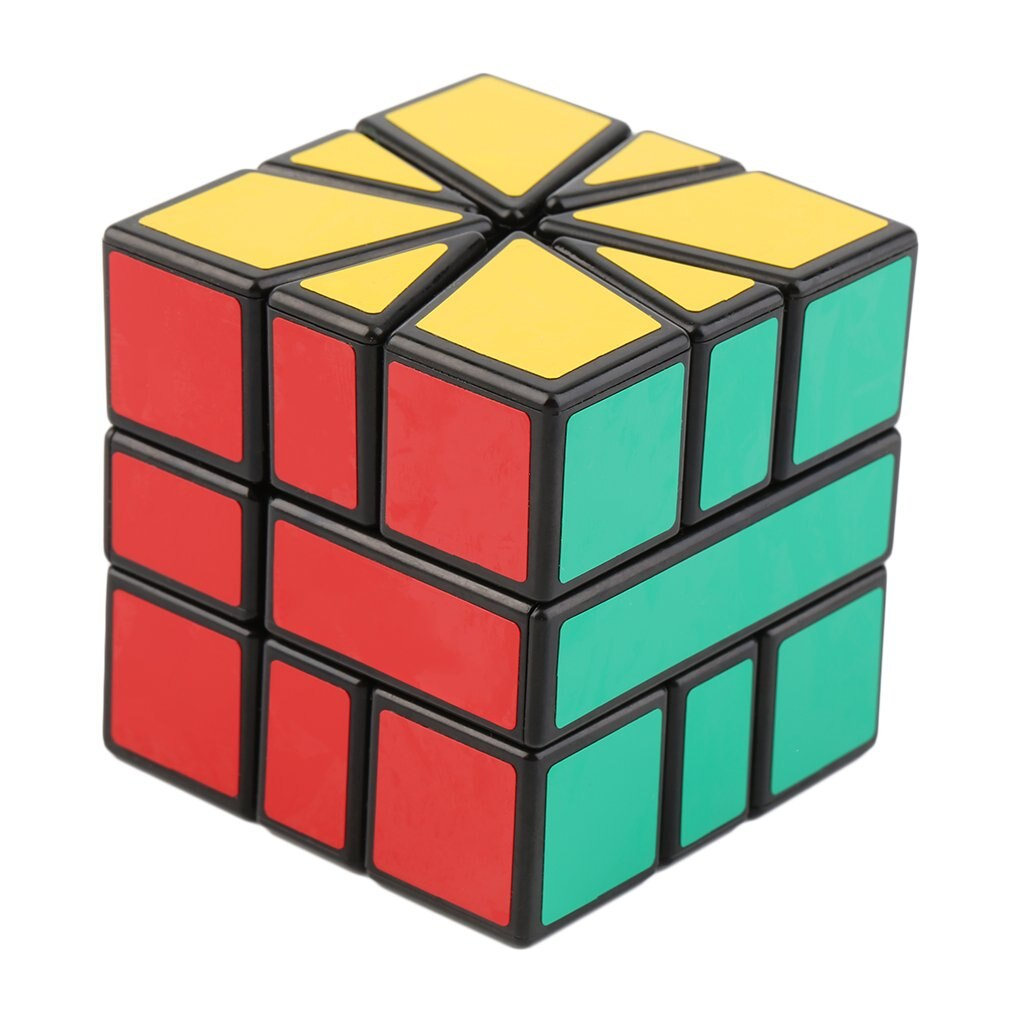
\includegraphics[width=0.8\textwidth]{assets/square1.jpg}}
                            \end{figure}
                    \end{columns}
                \end{frame}

        \subsection{non WCA}
            \begin{frame}{non WCA puzzles}
                \begin{figure}
                    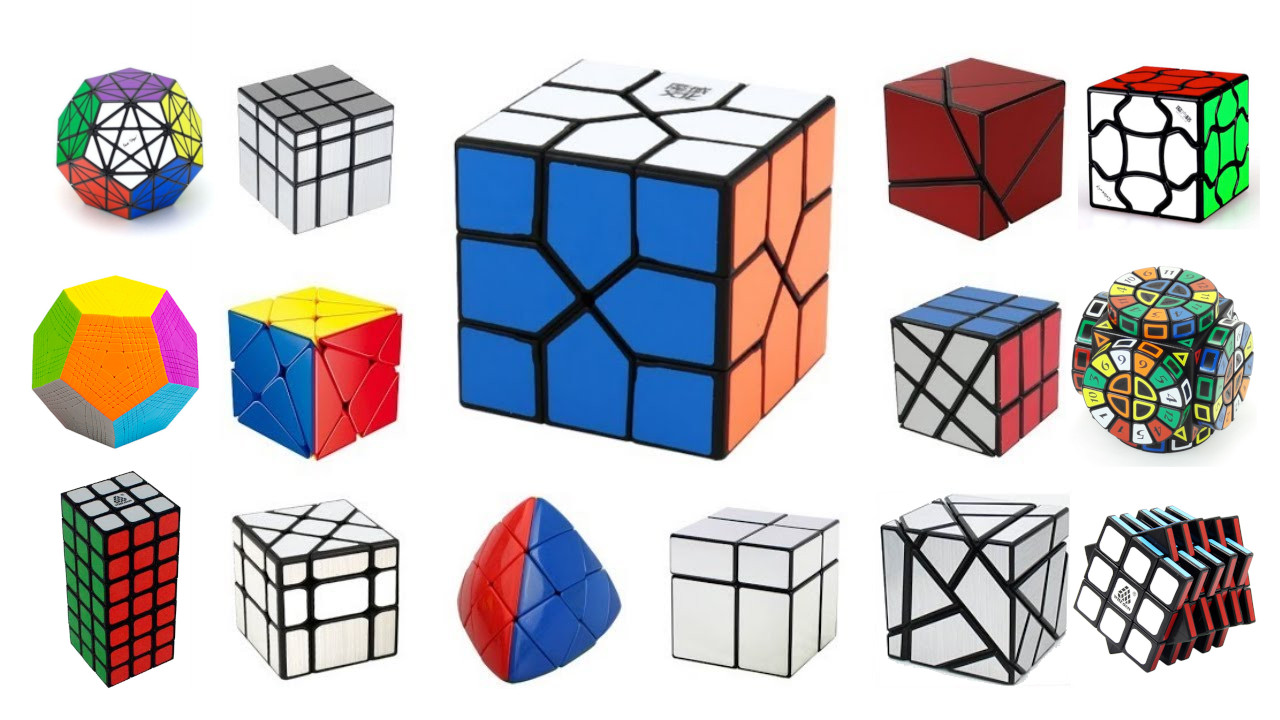
\includegraphics[width=\textwidth]{assets/nonWCAall.jpg}
                \end{figure}
            \end{frame}
        
    \section{Solving methods}
        \subsection{Beginners}
            \begin{frame}{Beginners method}
                \begin{columns}[t]
                    \column{.6\textwidth}
                    \newline \newline \newline 
                        \begin{itemize}
                            \item<2-> Slow $\rightarrow{}$ not meant for speedsolving \pause{}
                            \item<3-> Easy to learn \pause{}
                            \item<4-> Procedure:
                            \begin{enumerate}
                                \item<5-> Cross
                                \item<6-> First Layer
                                \item<6-> First two layers
                                \item<7-> Orient edges of LL
                                \item<9-> Permute edges of LL
                                \item<10-> Permute corners of LL
                                \item<11-> Orient edges of LL
                            \end{enumerate}
                        \end{itemize}
                    \column{.25\textwidth}
                        \begin{figure}
                            \visible<5->{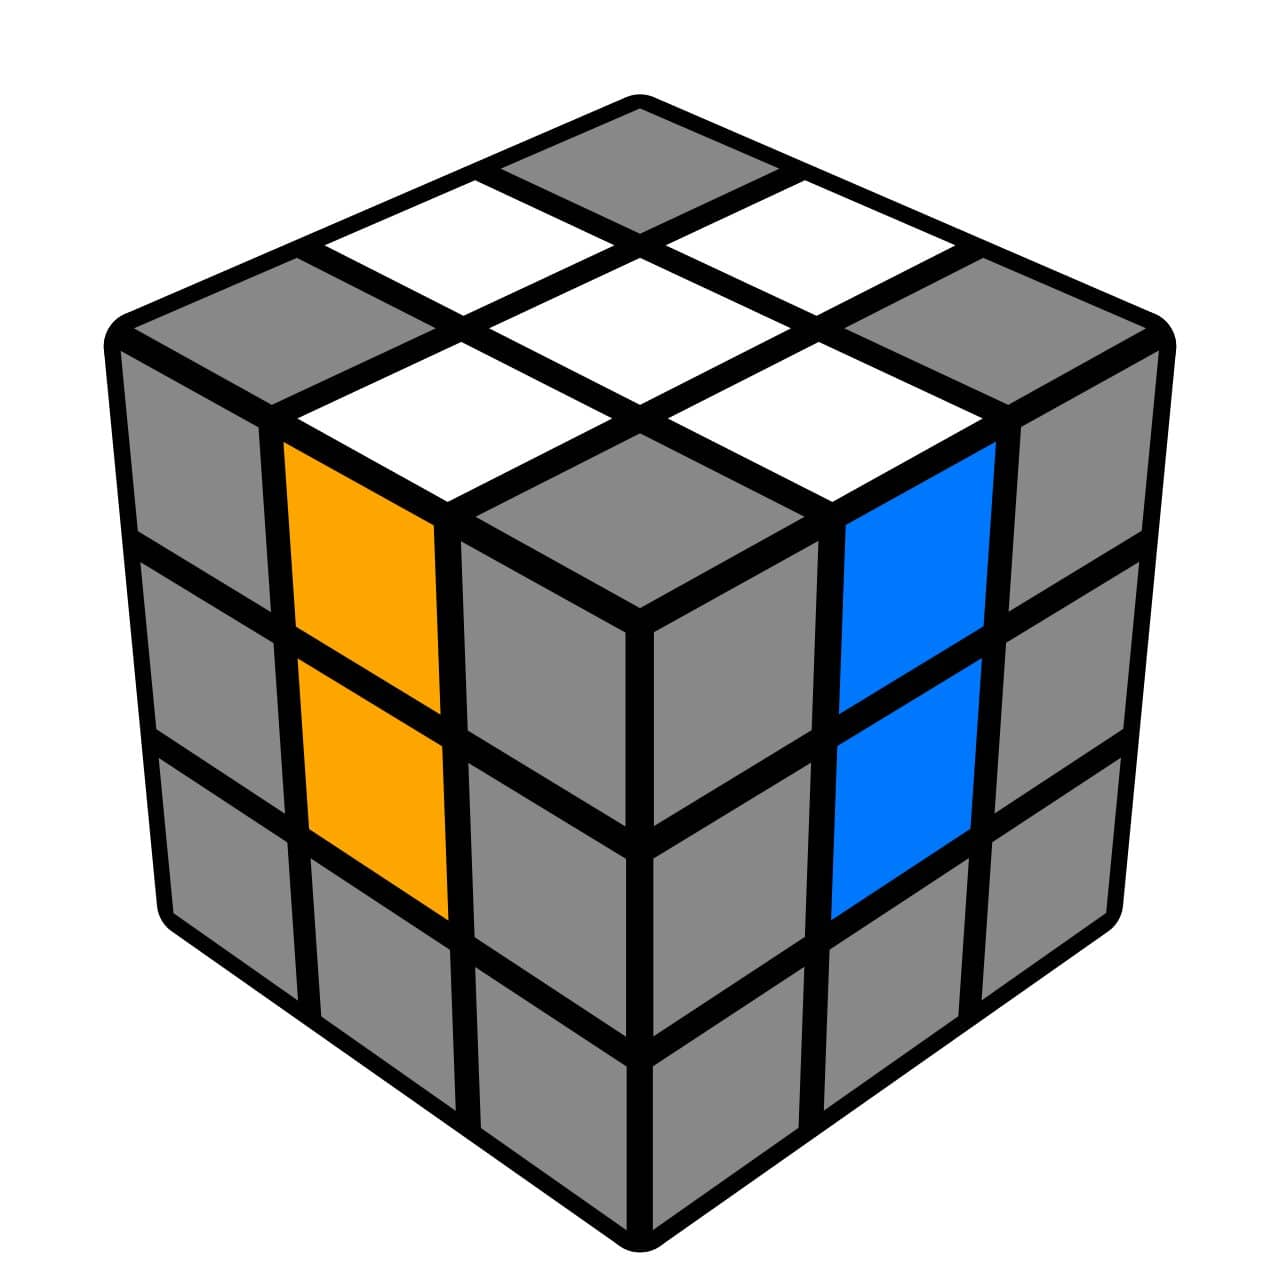
\includegraphics[width=.5\textwidth]{assets/cross.jpg}}
                            \visible<7->{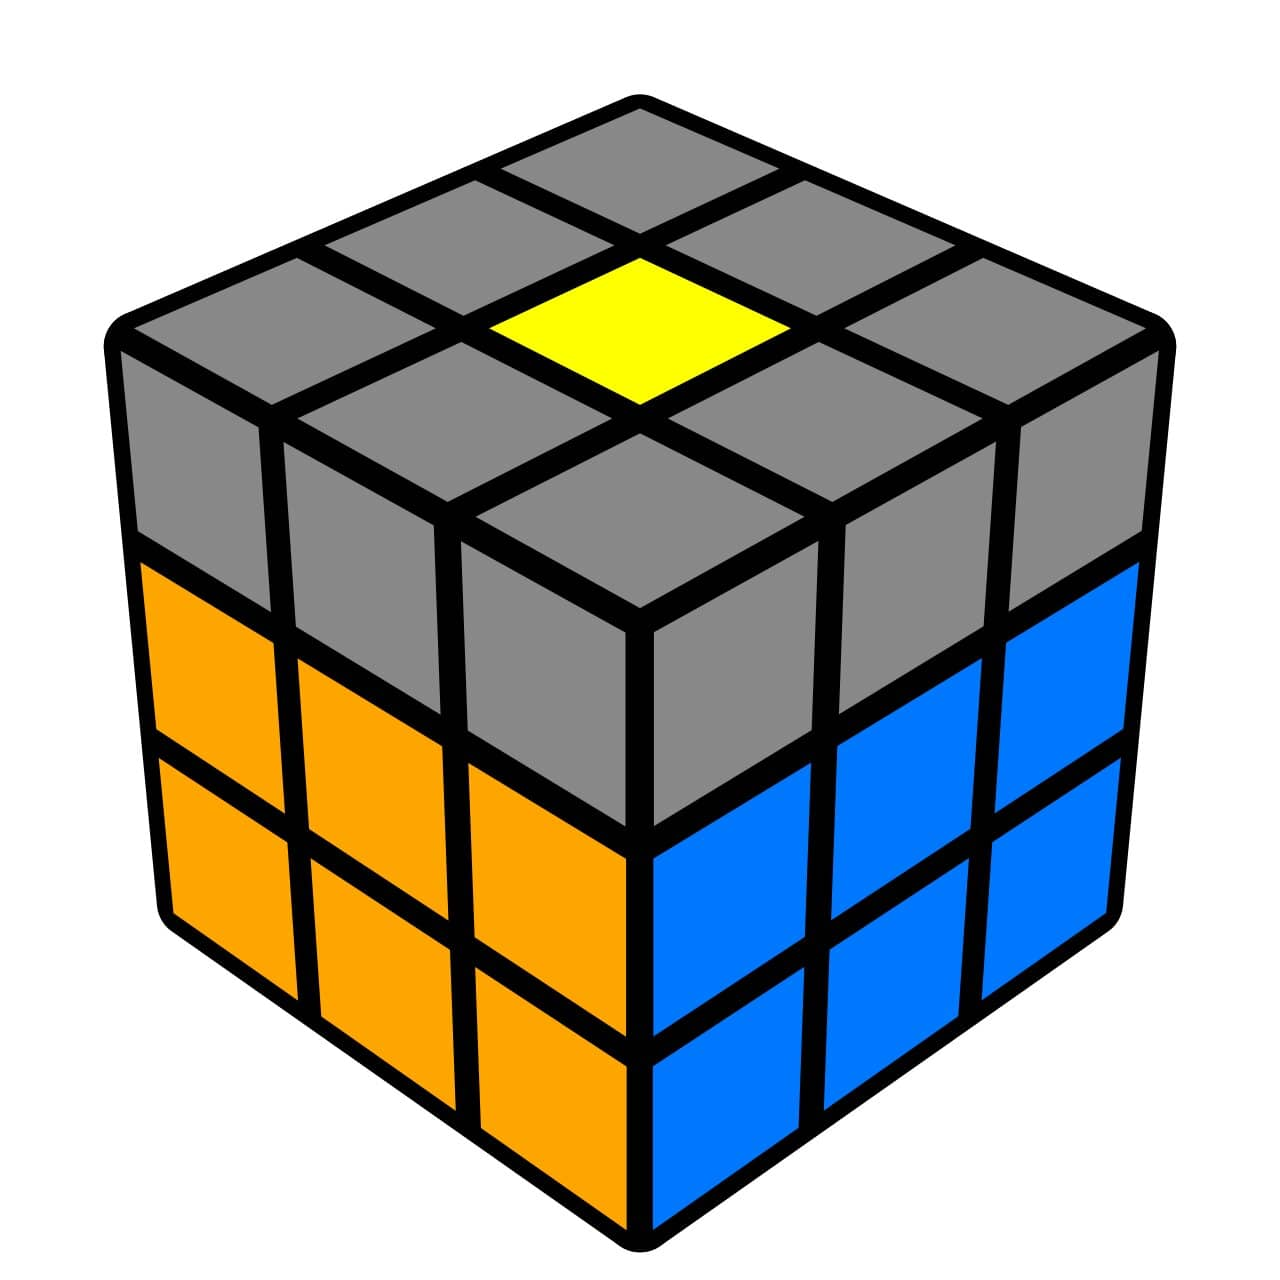
\includegraphics[width=.5\textwidth]{assets/f2l.jpg}}
                            \visible<9->{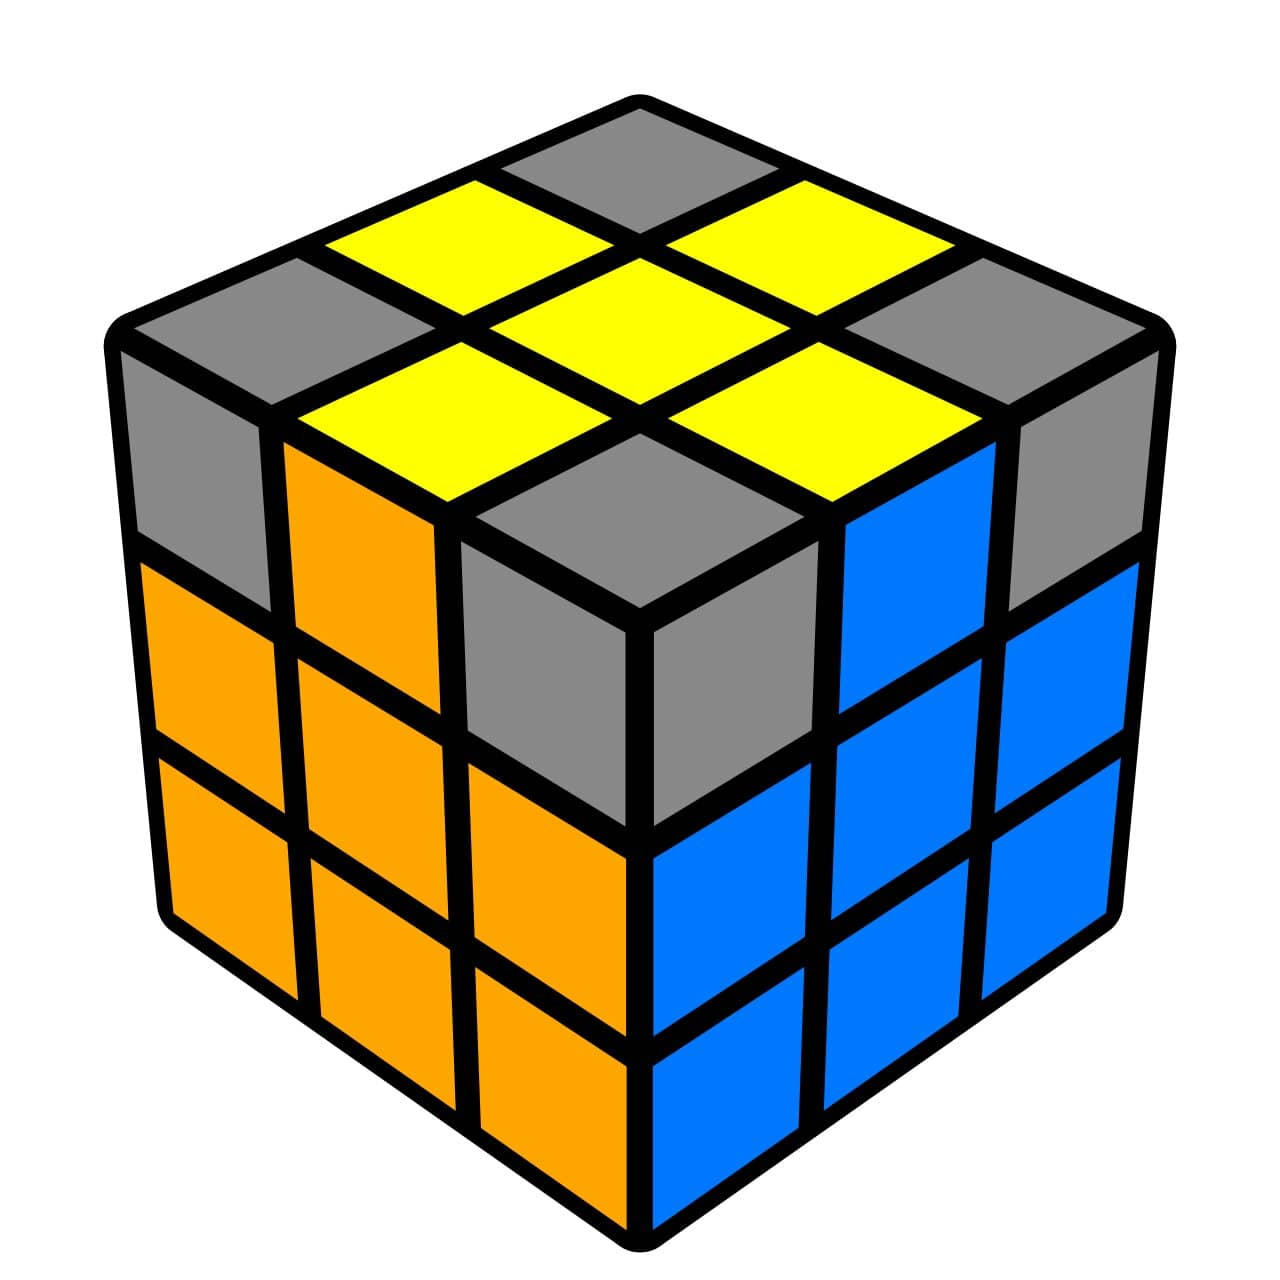
\includegraphics[width=.5\textwidth]{assets/oyellowcross.jpg}}
                            \visible<11->{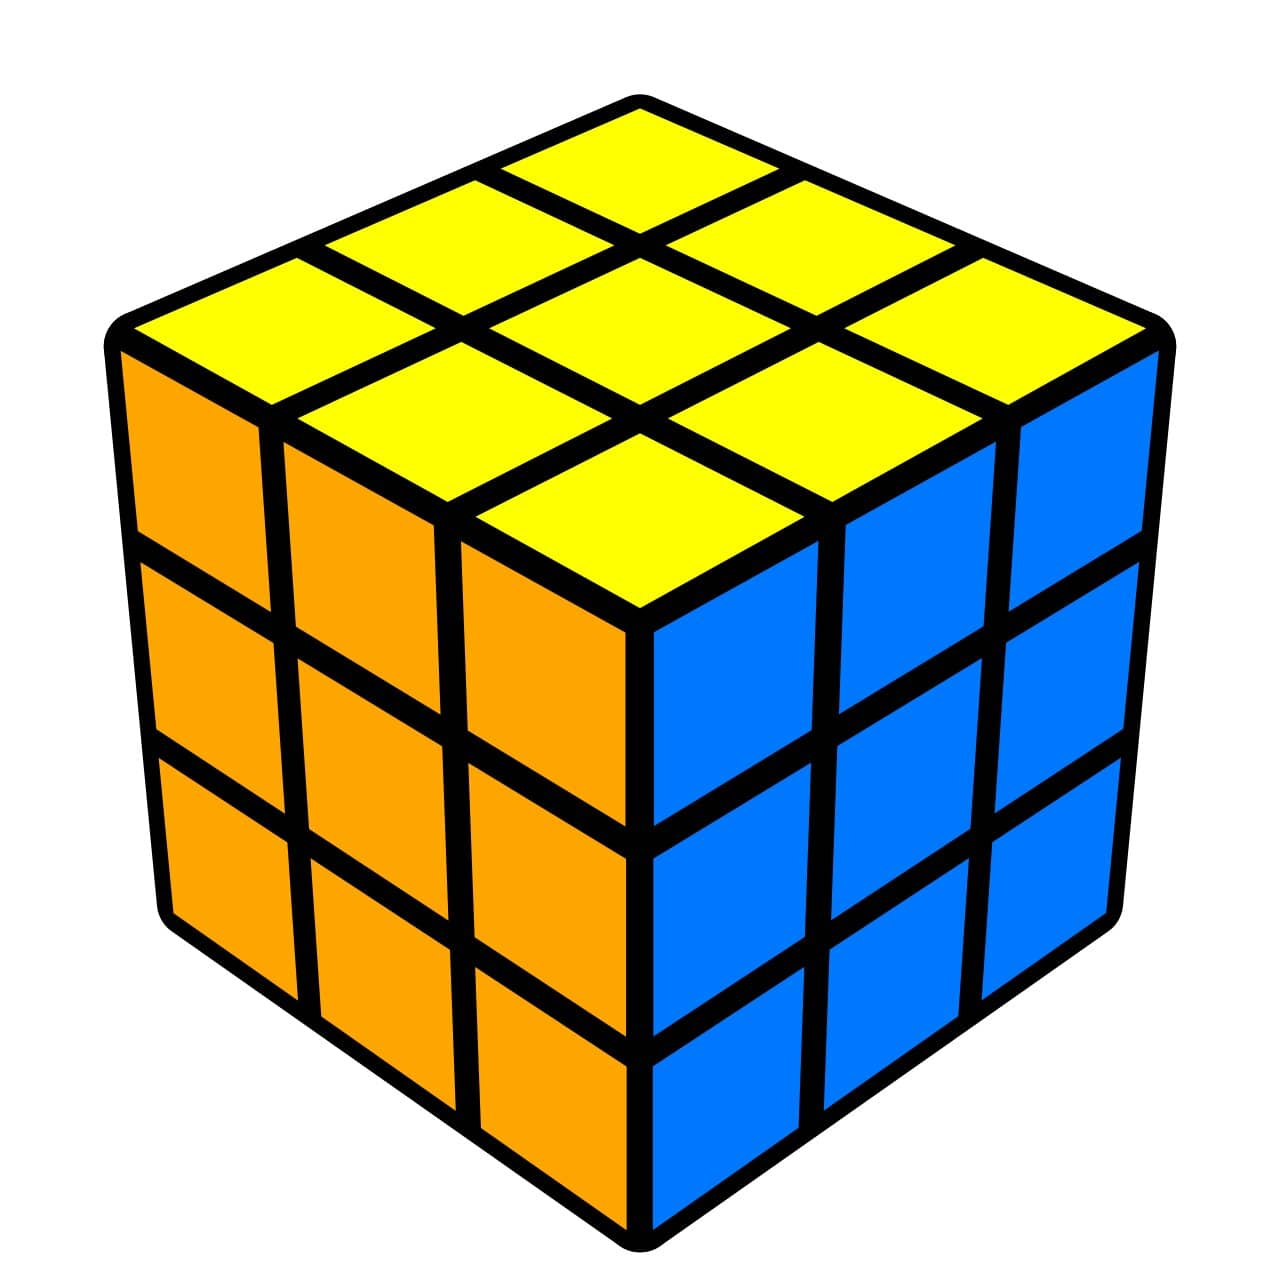
\includegraphics[width=.5\textwidth]{assets/oyellowcorners.jpg}}
                        \end{figure}
                    \column{.25\textwidth}
                        \begin{figure}
                            \visible<6->{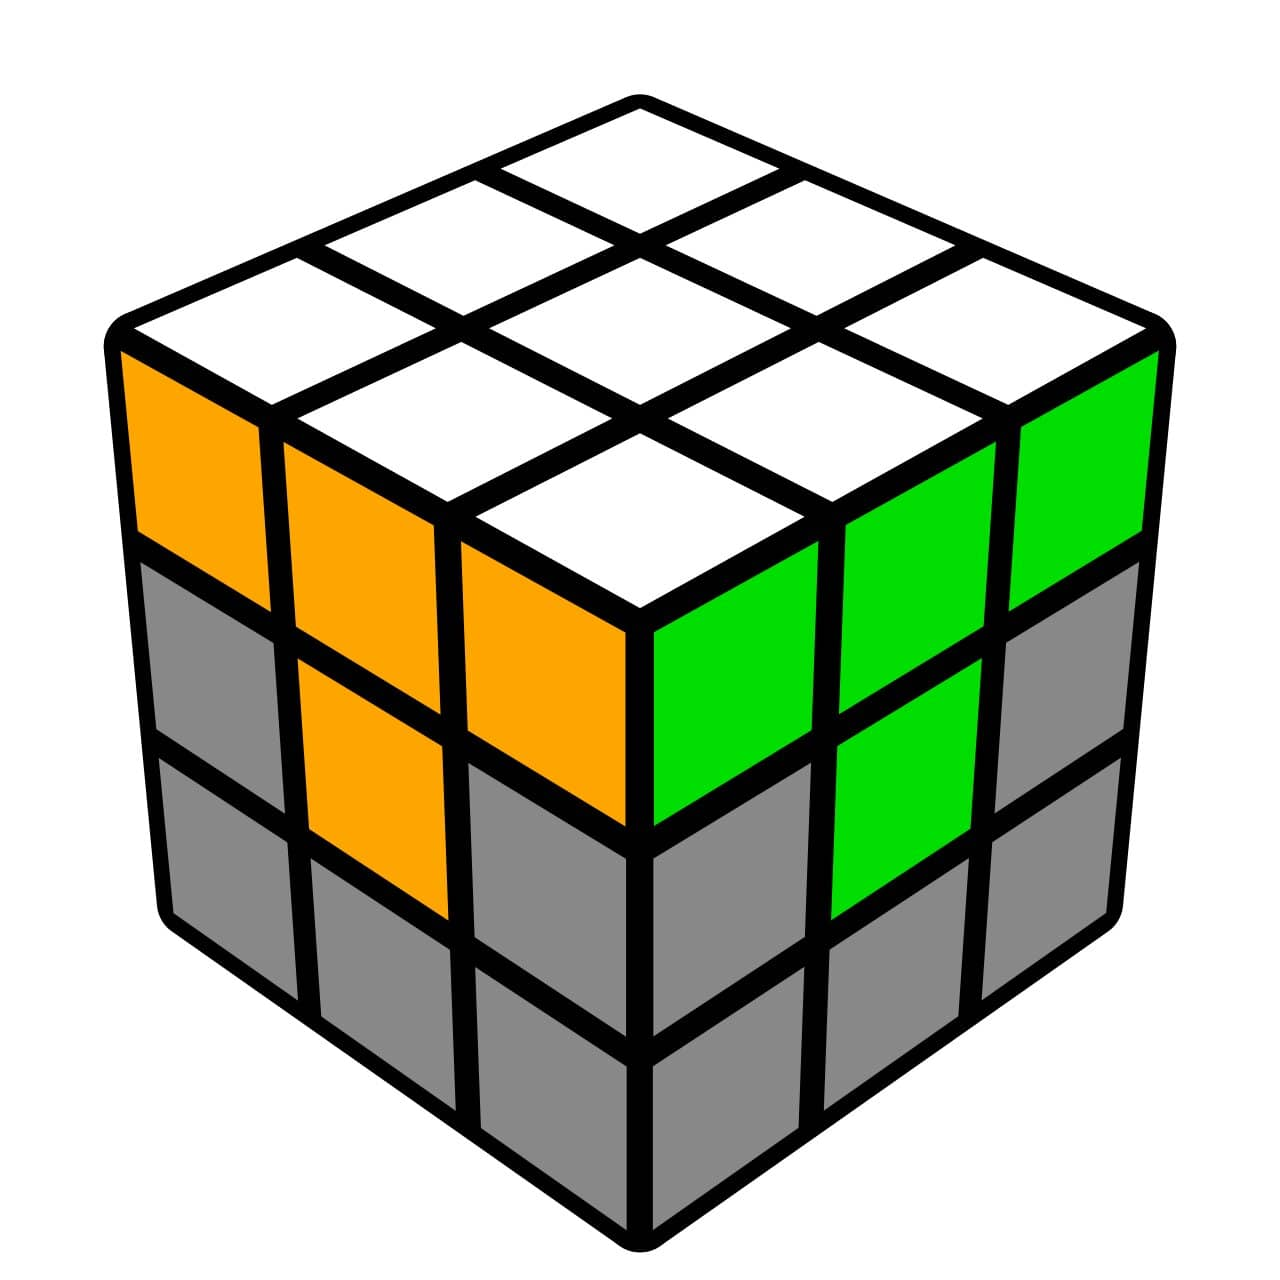
\includegraphics[width=.5\textwidth]{assets/f1l.jpg}}
                            \visible<8->{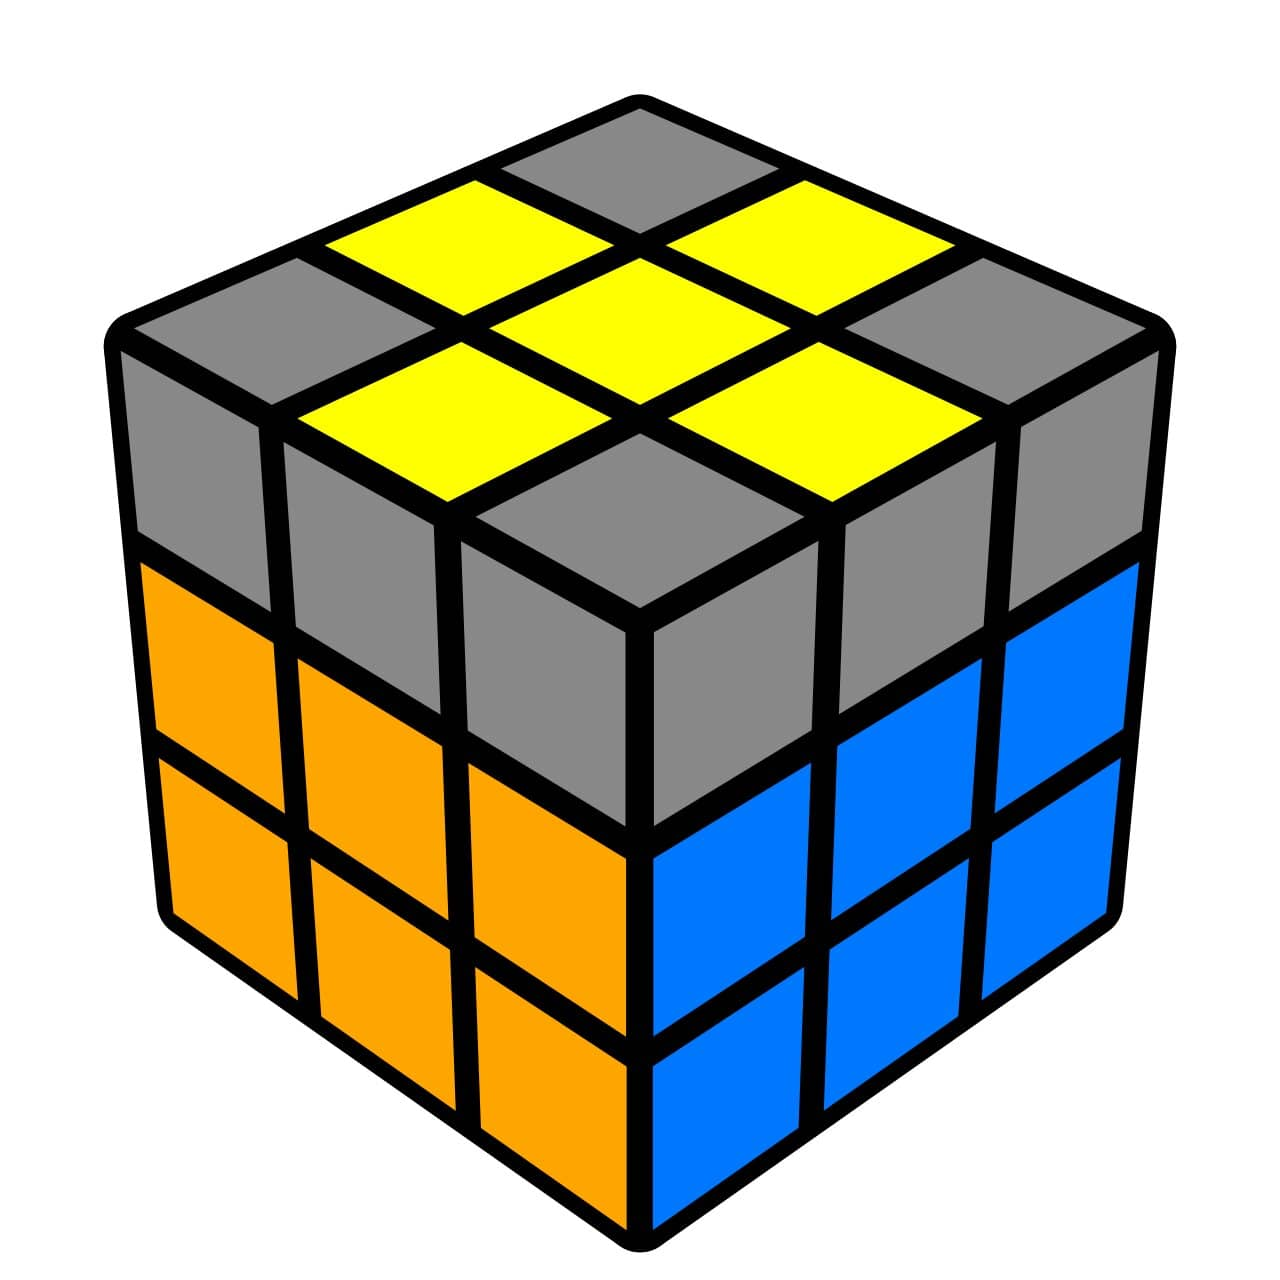
\includegraphics[width=.5\textwidth]{assets/yellowcross.jpg}}
                            \visible<10->{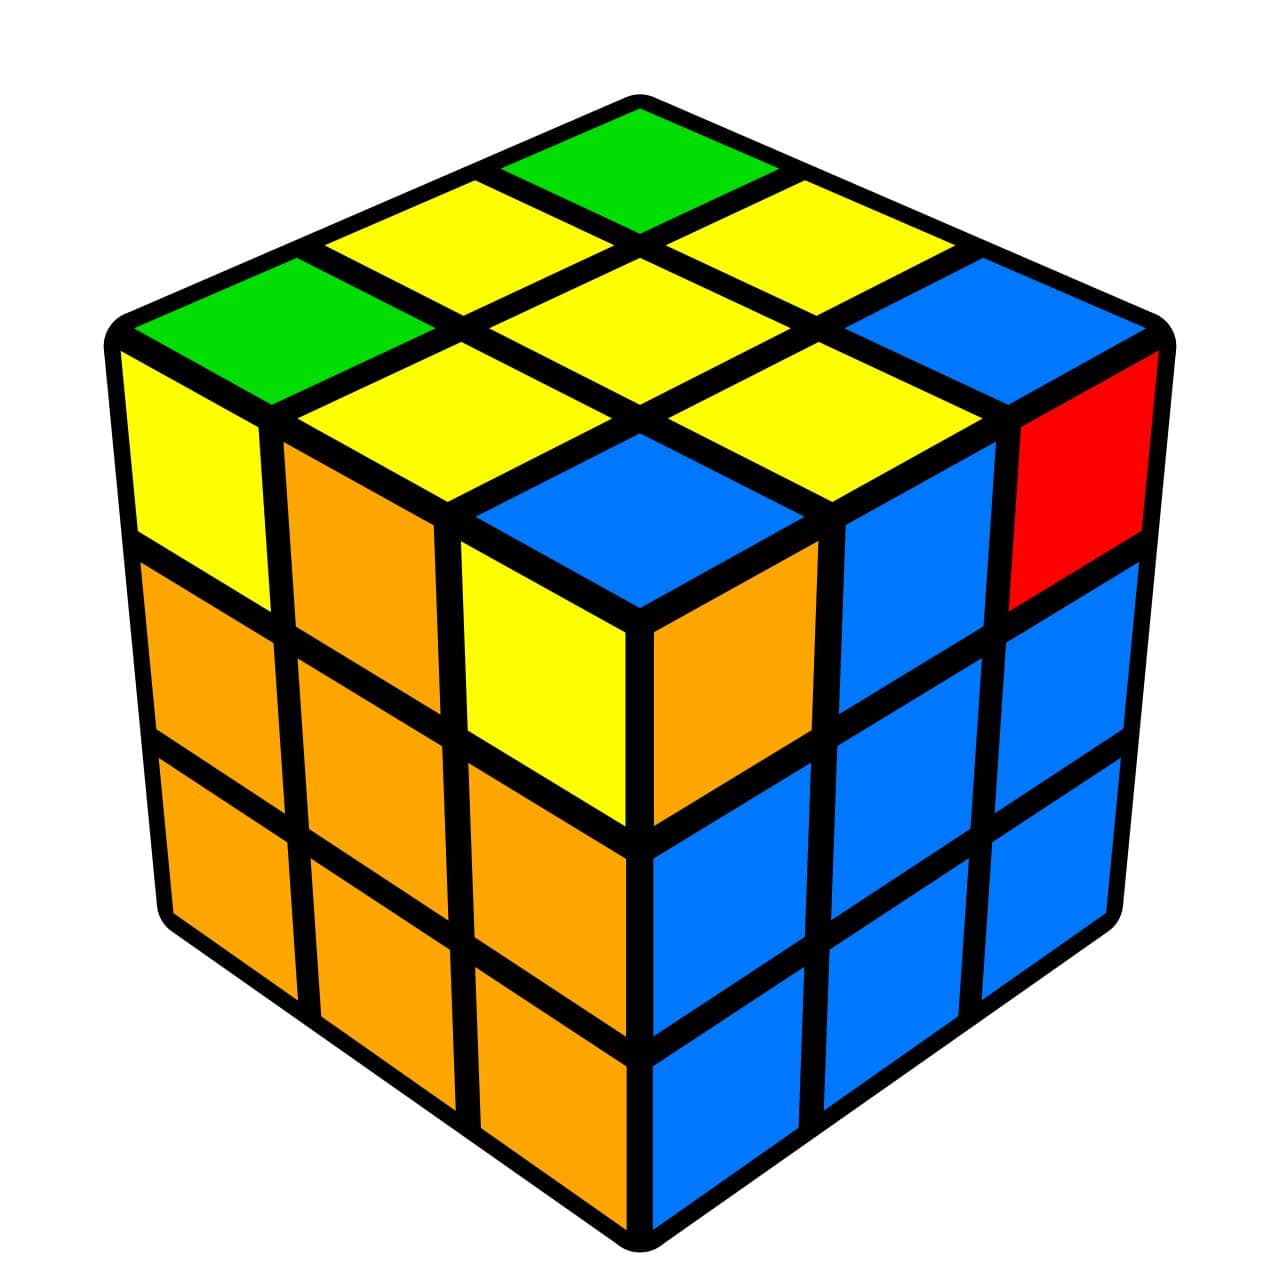
\includegraphics[width=.5\textwidth]{assets/pyellowcorners.jpg}}
                        \end{figure}
                \end{columns}
            \end{frame}
        \subsection{CFOP}
            \begin{frame}{CFOP method}
                \begin{columns}[c] 
                    \column{.6\textwidth} 
                        \begin{itemize}
                            \item<2-> Used by some of the best speedsolvers in the world \pause{}
                            \item<3-> Easy to learn
                            \item<4-> Procedure:
                            \begin{enumerate}
                                \item<5-> Cross
                                \item<6-> F2L
                                \item<7-> OLL
                                \item<8-> PLL
                            \end{enumerate}
                        \end{itemize}
                    \column{.25\textwidth} 
                        \begin{figure}
                            \visible<5->{\includegraphics[width=.6\textwidth]{assets/Cross.jpg}}
                            \visible<6->{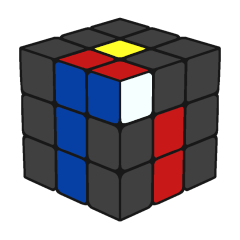
\includegraphics[width=.5\textwidth]{assets/F2L.png}}
                            \visible<7->{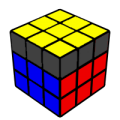
\includegraphics[width=.5\textwidth]{assets/OLL.png}}
                            \visible<8->{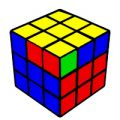
\includegraphics[width=.5\textwidth]{assets/PLL.jpg}}
                        \end{figure}
                \end{columns}
            \end{frame}
        \subsection{ROUX}
            \begin{frame}{ROUX method}
                \begin{columns}[c]
                    \column{.6\textwidth}
                        \begin{itemize}
                            \item<1-> Used by some of the best speedsolvers in the world
                            \item<2-> Quite intuitive 
                            \item<3-> Procedure:
                            \begin{enumerate}
                                \item<5-> first block
                                \item<6-> second Block
                                \item<7-> Orient and perumte corners of LL
                                \item<8-> Orient last edges
                                \item<9-> Permute last edges
                            \end{enumerate}
                        \end{itemize}
                    \column{.3\textwidth}
                        \begin{figure}
                            \visible<5->{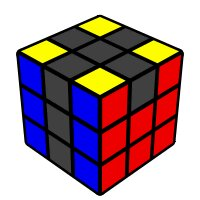
\includegraphics[width=\textwidth]{assets/ROUXmethod.jpg}}
                        \end{figure}
                \end{columns}
            \end{frame}
        \subsection{others}
            \begin{frame}{Other methods}
                \begin{itemize}
                    \pause{}
                    \item Kociemba $\rightarrow{}$ Computer \pause{}
                    \item ZZ $\rightarrow{}$ Speedsolving \pause{}
                    \item Petrus $\rightarrow{}$ Old speedsolving method \pause{}
                    \item Old Pochmann method $\rightarrow{}$ BLD \pause{}
                    \item 3-Style $\rightarrow{}$ BLD \pause{}
                    \item Variations of each one 
                \end{itemize}
            \end{frame}
    \section{What about me?}
        \begin{frame}{What about me?}
            \begin{itemize}
                \pause{}
                \item Started in November 2020 \pause{}
                \item Speedsolver \pause{}
                \item Main events: \pause{}
                \begin{enumerate}
                    \item 3$\times$3$\times$3 \pause{}
                    \item 3$\times$3$\times$3 OH \pause{}
                    \item 2$\times$2$\times$2 \pause{}
                \end{enumerate}
                \item Average around 16 seconds $\rightarrow$ Official Ao5 17.01 \pause{}
                \item PB 10.18s $\rightarrow$ Official PB 12.11\pause{}
                \item WCA ID $\rightarrow$ 2021LOFF01
            \end{itemize}
        \end{frame}
    \begin{frame}{}
        \centering \Large
        \emph{Thank you for listening}
        \end{frame}
\end{document}